\section{Auswertung}
\label{sec:Auswertung}
Jegliche Fehlerrechnung wurde mit der Python-Bibliothek uncertainties \cite{uncertainties} absolviert.
Trotz dessen sind die Formeln für die Unsicherheiten in den jeweiligen Abschnitten angegeben.
Allgemeine Rechnungen wurden mit der Python-Bibliothek numpy \cite{numpy} automatisiert. \\
Die Spannung $U_0$ beträgt bei allen Durchführungen $\SI{6.4}{\volt}$
\subsection{Bestimmung der Zeitkonstante mit dem Entladevorgang}
Die während der Durchführung gemessenen Werte für $U_\text{C}$ in Abhängigkeit von der Zeit sind in Tabelle \ref{tab:UCt} aufgeführt.
\begin{table}
    \centering
    \caption{Gemessene Kondensatorspannung $U_\text{C} \left (t \right )$}
    \label{tab:UCt}
    \begin{tabular}{S[table-format=1.1] S[table-format = 1.1]}
        \toprule
        {$ t \mathbin{/} \si{\milli\second}$} & {$U_\text{C} \mathbin{/} \si{\volt}$} \\
        \midrule
        0   & 6.2 \\
        0.1 & 5.3 \\
        0.2 & 4.7 \\
        0.3 & 4.1 \\
        0.4 & 3.5 \\
        0.5 & 2.9 \\
        0.6 & 2.5 \\
        0.7 & 1.9 \\
        0.8 & 1.5 \\
        0.9 & 1.1 \\
        1   & 0.7 \\
        1.1 & 0.5 \\
        1.2 & 0.1 \\
        \bottomrule        
    \end{tabular}
\end{table}
\begin{figure}
        \centering
        \caption{Verlauf der Spannung bei einem Entladevorgang}
        \label{fig:discharge}
        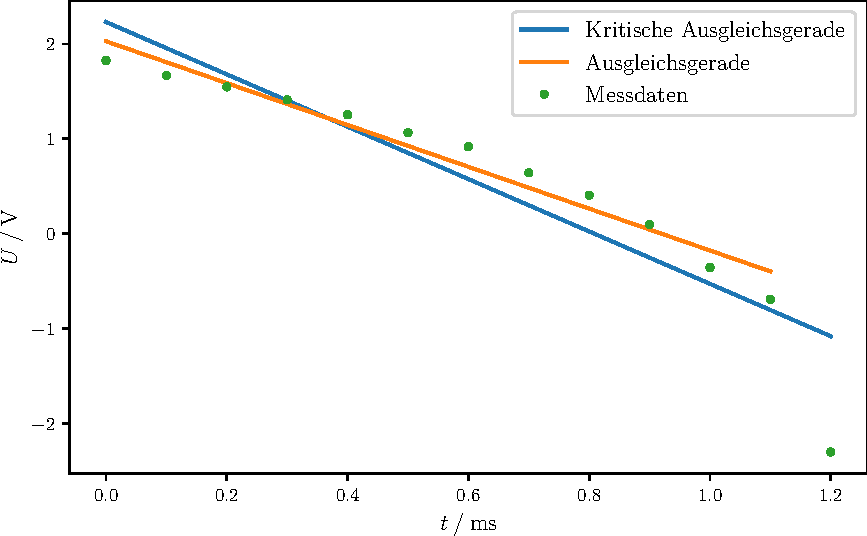
\includegraphics{build/uct.pdf}
\end{figure}
\noindent Bei dem Spannungsverlauf in Abblidung \ref{fig:discharge} ist zunächst anzumerken, dass dort zwei Ausgleichsgeraden angelegt wurden. 
Dies liegt der Ursache zu Grunde, dass der letzte Punkt der Messreihe einen sehr starke Abweichung zeigt.
Die gesamte Ausgleichsgerade beschreibt die komplette Messreihe, wobei der letzte Messwert bei der kritischen Ausgleichsgerade ausgelassen wurde.
Im Folgenden werden die Rechungen mit den Parametern der kritischen Ausgleichsgeraden durchgeführt.
Für die Bestimmung der Zeitkonstante $RC$ wird Geleichung \eqref{eqn:Charge} verwendet.
Jedoch wird die Ladung $Q$ durch die Spannung $U_\text{C}$ ersetzt.
Umgestellt und logarithmiert ergibt sich 
\begin{equation}
    \ln \left( \frac{U_\text{C}}{U_0} \right ) =  - \frac{t}{RC} \; \text{.} 
\end{equation} 
Die Ausgleichsgerade hat die Form $ \ln \left( \sfrac{U_\text{C}}{U_0} \right ) = at + b$, wobei $a = - \sfrac{1}{RC}$ gilt.
Die Parameter haben die Werte 
\begin{align*}
    a &= \SI{-0.3447(229)}{\per\milli\second} \\
    b &= \num{0.3169(149)} \; \text{.}
\end{align*}
Der Wert für $a$ in $RC = - \sfrac{1}{a}$ eingesetzt ergibt
\begin{equation*}
    \tau = RC = \SI{2.90(19)}{\milli\second} \; \text{.}
\end{equation*}
\subsection{Frquenzabhängige Spannunsgmessung}
\begin{figure}
    \centering
    \caption{Kondensatorspannung $U_\text{C} \left( \omega \right)$}
    \label{fig:ucw}
    \includegraphics{build/ucw.pdf}
\end{figure}